\subsection{When are random effects useful?}
\label{sec:whenrandomeffectsareuseful}

\subsubsection{Introduction to random effects}
\label{sec:introductiontorandomeffects}

% \textit{Generalised Linear Models} (GLMs), as discussed in the previous chapter, allow us to estimate the effects which various \textit{predictors} or \textit{regressors} (\ie corpus linguistic variables) have on an \textit{outcome} or \textit{response} (\ie another corpus linguistic variable).
% Surely, the most typical application (in corpus linguistics) is the modeling of \textit{alternations}, \ie phenomena where the response variable of interest encodes a choice of forms or constructions, for example a case alternation (a binary or multi-valued categorical response), alternations of graphemic forms such as contracted vs.\ non-contracted, ordering preferences such as the order of prenominal adjectives, or syntactic\slash constructional alternations such as the dative alternation.%
% \footnote{In this article, I restrict the discussion to GL(M)Ms with categorical responses, simply because the continuous responses in Linear (Mixed) Models -- or LM(M)s – are not found very often in corpus linguistics.
% Also, an L(M)M can be understood as a GL(M)M with an identity link function and a Gaussian distribution for the residuals.}
% The approach is called \textit{generalised} in contrast to normal linear models because the response need not be numerical, and the \textit{errors} or \textit{residuals} do not have to be (approximately) normally distributed.
% First, this is achieved by allowing for different types of exponential distributions for the residuals, which requires the use of a more general estimator than least-squares, typically likelihood maximisation.
% Second, \textit{link functions} are introduced which relate the additive linear term that combines the predictors in a non-linear way to the response variable.
(Generalised) Linear Mixed Models (GLMMs) are an extension of (Generalised) Linear Models (GLMs).
They add what are often called \textit{random effects} and \textit{mix} them with the normal predictors (\textit{fixed effects}) as used in GLMs.
Alternatively, statisticians speak of \textit{multilevel models} or \textit{hierarchical models} \citep{GelmanHill2006}, a terminology to be explained in Section~\ref{sec:hierarchicalormultilevelmodels}.

The purpose of including random effects is usually said to be the modeling of variance between groups of observations.
A single observation (or \textit{data point} or \textit{measurement} or \textit{unit}) is one atomic exemplar entering into the statistical analysis of a study.
In corpus linguistics, single observations can be understood as single lines in a concordance.
These concordance lines could contain, for example, clauses or sentences in which one of the alternants of a morpho-syntactic alternation occurs, the goal being to model the influence of diverse properties of the clauses sentences on the choice of the alternants.
Along similar lines and under a similar research question, they could contain occurrences of a contracted or a non-contracted form of words (like \textit{am} and \textit{'m} in English).
As a another example, the concordance lines could contain NPs where two pre-nominal adjectives are used, the goal being to determine the factors influencing their relative ordering.
When such observations are grouped, it is often plausible to assume that there is some variance in the choice of the alternating forms or constructions at the group-level.
If this is the case and the grouping factor is not included in the model, the error terms within the groups will be correlated.
Put simply, this means that means of the group-wise errors will be different.
Since the estimators used for estimating the parameters of GLMs work under the assumption of non-correlated errors, standard errors for model coefficients will typically be estimated as smaller than they nominally are, leading to increased Type I error rates in inferences about the coefficients.%
\footnote{Type I errors occur when the null hypothesis is rejected although it is true.
The requirement that error should be uncorrelated is often called ``independence (of errors)''.}
This gets even worse when there are within-group tendencies regarding the direction and strength of the influence of the other regressors, \ie when there is an interaction between them and the grouping factor (\eg \citealt{SchielzethForstmeier2009}).
This is why known variation by group should always be accounted for in the model.
Random effects are often a convenient way to do so.

Groups can be defined by any linguistically relevant grouping factor, such as the individual speakers (or authors, writers, etc.), the regions where they were born or live, social groups with which they identify, but also time time periods, genres, styles, etc.
% If the concordance in a study contains, say, ten exemplars each written by ten speakers, then the speaker grouping factor has ten levels and defines ten groups.
% We know that preferences vary between speakers, and it is therefore reasonable to take care of this variance in our statistics in some way.
% The same goes for the other possible groups just mentioned.
Specific lexemes often have idiosyncratic affinities towards alternants in alternating constructions.
Therefore, exemplars containing specific lexemes also constitute groups.
In cases like the dative alternation individual verbs co-occur with the alternants to different degrees.
%  with considerable between-group variance.
% As an example from outside corpus linguistics, variation between participants is modeled by including a random effect for speaker in experimental settings.

% While random effects are often presented like this using conceptual arguments,
The crucial question in specifying models is not whether to include these grouping factors at all, but rather whether to include them as fixed effects or as random effects.
Random effects structures are very suitable for accounting for group-level variation in regression, but while formulaic recommendations such as ``Always include random effects for speaker and genre!'' provide useful guidance for beginners, the choice between fixed and random effects can and should be made based on an analysis and understanding of the data set at hand and the differences and similarities in the resulting models.
The remainder of Section~\ref{sec:whenrandomeffectsareuseful} introduces three important points to consider about the structure of the data typically used in mixed modeling.
% This is intended to show readers that mixed or multilevel\slash hierarchical modeling is simply a matter of doing justice to the structure of the data.
Then, Section~\ref{sec:modelspecificationandmodelingassumptions} provides a moderately technical introduction to modeling.
Section~\ref{sec:specifyingmodelsusinglme4inr} shows how mixed models are specified using the \texttt{lme4} package in \texttt{R}, and Section~\ref{sec:afterfittingmodelswithlme4} deals with the interpretation of the output.


\subsubsection{Crossed and nested effects}
\label{sec:crossedandnestedeffects}

\begin{table}
  \centering
  \begin{tabular}{lll}
    \toprule
    \textbf{Exemplar} & \textbf{Speaker}  & \textbf{Region}        \\
    \midrule
                    1 &           Daryl  &         Tyneside       \\
                    2 &           Daryl  &         Tyneside       \\
                    3 &           Riley  &         Tyneside       \\
                    4 &           Riley  &         Tyneside       \\
                    5 &           Dale   &         Greater London \\
                    6 &           Dale   &         Greater London \\
                    7 &           Reed   &         Greater London \\
                    8 &           Reed   &         Greater London \\
    \bottomrule
  \end{tabular}
  \caption{Illustration of nested factors}
  \label{tab:nested}
\end{table}

% It was established in the previous section that random effects are a means of accounting for group-level variance in regression models.
% This section briefly introduces a distinction that plays a role in modeling when there is more than one grouping factor (to be used either as a fixed or random effect).
This section discusses a distinction that arises when there is more than one grouping factor.
When this is the case, each pair of grouping factors can be \textit{nested} or \textit{crossed}.
By way of example, we can group exemplars (such as sentences) by the individual speakers who wrote or uttered them, and we can group speakers by their region of birth.
Such a data set would intrinsically be \textit{nested}, as Table~\ref{tab:crossed} illustrates.
Since speakers have a unique region of birth, Tyneside is the unique \textit{region} value for the speakers Daryl and Riley, and Greater London is the unique \textit{region} value for Dale and Reed.
% There cannot be exemplars where, for example, the speaker is Daryl and the region is Greater London (assuming that speakers are uniquely identified by the labels in the middle column).
In this example, the region factor nests the speaker factor.
This example was chosen because the nesting is conceptually necessary.
However, even when a data set has a nested structure by accident, standard packages in \texttt{R} will also treat them as nested
%, and a closer look at data sets should be part of any protocol for using GLMMs in corpus studies
(see Section~\ref{sec:specifyingmodelsusinglme4inr}).

When the grouped entities (themselves groups) do not uniquely belong to levels of the grouping factor, the factors are \textit{crossed}.
Continuing the example, crossed factors for speaker and mode are illustrated in Table~\ref{tab:crossed}.
%
\begin{table}
  \centering
  \begin{tabular}{lll}
    \toprule
    \textbf{Exemplar} & \textbf{Speaker}  & \textbf{Mode}   \\
    \midrule
                    1 &           Daryl  &         Spoken  \\
                    2 &           Daryl  &         Written \\
                    3 &           Riley  &         Spoken  \\
                    4 &           Riley  &         Spoken  \\
                    5 &           Dale   &         Written \\
                    6 &           Dale   &         Written \\
                    7 &           Reed   &         Spoken  \\
                    8 &           Reed   &         Written \\
    \bottomrule
  \end{tabular}
  \caption{Illustration of crossed factors}
  \label{tab:crossed}
\end{table}
%
While there are only spoken sentences by Riley and only written sentences by Dale in the sample, there is one spoken and one written sentence each by Daryl and Reed.
There is a many-to-many relation between speakers and modes, which is characteristic of crossed factors.
In Table~\ref{tab:nested}, the relation between speakers and regions is many-to-one, which is typical of nested factors.
% In experimental settings, the design often makes sure that the combinations of nested or crossed factors are represented by equal numbers of observations (such that, for example, there is an equal number of written and spoken sentences from each speaker).
% Contrarily, the situation in Table~\ref{tab:crossed} is typical of corpus studies where pseudo-random sampling from a pre-compiled corpus such as the BNC was used.
% This does not affect the practical modeling procedures much, especially when random factors are used, as will be shown below.
% However, practitioners must be aware of it when interpreting the data.

% Finally, it should be noted that grouping factors can form hierarchical structures.
With more than two grouping factors, there can be more than one level of nesting.
Mode could nest genre if genres are defined such that each genre is either exclusively spoken or written.
%, and in a given corpus, speakers might be nested within genres because each of them only contributed material to one genre.%
%\footnote{In this example, the second level of nesting is not a conceptual necessity.
%In fact, it would be quite surprising if the real world were shaped like this.
%However, standard corpus compilation techniques might easily lead to a situation where exactly this is the case, simply because it is often difficult to sample texts and utterances from single speakers across a wide range of genres.}
Similarly, in a study on adjectives we might want to describe adjectives as being either intersective or non-intersective.
Within the two groups, a finer-grained semantic classification might be nested, which itself nests single adjective lexemes.
However, not all of these structures should be modeled as nested random effects.
In the latter case, for example, the low number of levels in one factor (intersectivity with just two levels) predestines it as a second-level predictor rather than a nesting factor; see Section~\ref{sec:hierarchicalormultilevelmodels}.

\subsubsection{Hierarchical or multilevel modeling}
\label{sec:hierarchicalormultilevelmodels}

% This section introduces the idea that so-called random effects actually introduce new levels of modeling, or \textit{secondary models}.
% It is argued that this is not a technical matter but required by the structure of certain data sets.
This section describes the types of data to be used in true multilevel models.
Let us assume that we wanted to account for lexeme-specific variation in a study on an alternation phenomenon such as the dative alternation in English by specifying the lexeme as a random effect in the model.
Additionally, we suspect or know that a lexeme's overall frequency influences its preferences for occurring in the construction alternants.
% Now, we could simply quantise the frequency variable and turn it into an ordinal variable (for example in the form of frequency bands) and interpret it as a grouping factor which nests the lexeme grouping factor.
% However, frequency obviously is a numerical and not a categorical variable, and by using it as a grouping factor we would destroy valuable information.
A similar situation would arise in a study of learner corpus data (even of the same alternation phenomenon) with a learner grouping factor if we also knew that the number of years learners have learned a language influences their performance with regard to a specific phenomenon.
In such cases, variables like \textit{frequency} and \textit{number of learning years} are constant for each level of the grouping factor (\textit{lexeme} and \textit{learner}, respectively).
In other words, each lexeme has exactly one overall frequency, and each learner has had a fixed number of years of learning the language.%
\footnote{In the given example, things would get more complicated if the corpus contained observations of single learners at different points in time.
We simplify the scenario for the sake of an easier-to-follow introduction.
See also the last subsection of Section~\ref{sec:morecomplexmodels}.}

\begin{table}
  \centering
  \begin{tabular}{llllll}
    \toprule
    \multicolumn{3}{l}{\textbf{Level of observations}}          & \multicolumn{2}{l}{\textbf{Group level}}  & \textbf{Outcome} \\
    \textbf{Exemplar} & \textbf{Givenness} & \textbf{NP length} & \textbf{Verb} & \textbf{Verb freq.}       & \textbf{Alternant}\\
    \midrule
            1 &     New   &      8    &    give   &   6.99   & 1 \\
            2 &     Old   &      7    &    give   &   6.99   & 1 \\
            3 &     Old   &      5    &    give   &   6.99   & 2 \\
            4 &     Old   &      5    &    grant  &   5.97   & 2 \\
            5 &     New   &      9    &    grant  &   5.97   & 1 \\
            6 &     Old   &      6    &    grant  &   5.97   & 2 \\
            7 &     New   &      11   &   promise &   5.86   & 2 \\
            8 &     New   &      10   &   promise &   5.86   & 1 \\
            9 &     Old   &      9    &   promise &   5.86   & 2 \\
    \bottomrule
  \end{tabular}
  \caption{Illustration of a fictional data set which requires multilevel modeling; NP length could be measured in words; the lemma frequencies are actual logarithm-transformed frequencies per one million tokens taken from ENCOW14A \citep{SchaeferBildhauer2012}; the outcome column encodes whether alternant 1 or 2 was chosen}
  \label{tab:multilevel}
\end{table}

Such variables are thus reasonably interpretable only at the group-level.
Table~\ref{tab:multilevel} illustrates such a data set (fictional in this case).
It might be a small fraction of the data used to predict whether a ditransitive verb is used in the dative shift construction or not.
% The exemplar indices, again, simply identify single sentences containing one of the constructions of interest.
The givenness and the NP length status vary at the level observations.
To capture verb lemma specific tendencies, a verb lemma grouping factor is added.
The verb lemma frequency necessarily varies at the group level because each lemma has a unique frequency.
In such cases, an adequately specified multilevel model uses the group-level variables to partially predict the tendency of the grouping factor.
Put differently, the idiosyncratic effect associated with a lexeme, speaker, genre, etc.\ is split up into a truly idiosyncratic preference and a preference predictable from group-level variables.
This is achieved by specifying a second (linear) model which predicts the group-level random effect itself.
% , and the second-level predictor is a fixed effect in this model.
Such second-level models can even contain modeled effects themselves, giving rise to third-level models, and so on.
The data look similar to multilevel nesting, but (1) second-level models can account for continuous numerical predictors at the group-level, which nesting cannot, and (2) there might be situations where specifying even categorical second-level grouping factors as fixed effects in a second-level model is more appropriate than adding nested random effects (see Section~\ref{sec:modelspecificationandmodelingassumptions}).

As in the case of nested vs.\ crossed factors, standard packages in \texttt{R} usually take care of hierarchical modeling automatically, given that the data are structured and are specified accordingly.
This might, however, lead to situations where practitioners specify multilevel models without even knowing it, which in turn can lead to misinterpretations of the results.
See Section~\ref{sec:specifyingmodelsusinglme4inr} for details.
% Therefore, multilevel modeling will be introduced as the more general framework for so-called mixed effects models in Sections~\ref{sec:modelspecificationandmodelingassumptions} and \ref{sec:specifyingmodelsusinglme4inr}.

\subsubsection{Random slopes as interactions}
\label{sec:randominterceptsandslopes}

% Before moving on to the more technical discussion of hierarchical model specification in Section~\ref{sec:modelspecificationandmodelingassumptions}, one more basic concept will be discussed in this section, namely
This section introduces the data patterns that gives rise to \textit{varying intercepts} and \textit{varying slopes}. 
Varying intercepts are an adequate modeling tool when the overall tendency in the outcome variable changes with the levels of the grouping factor.
% It is shown that random slopes are just another way of modeling an interaction between influencing factors.

\begin{figure}[!htpb]
  \centering
  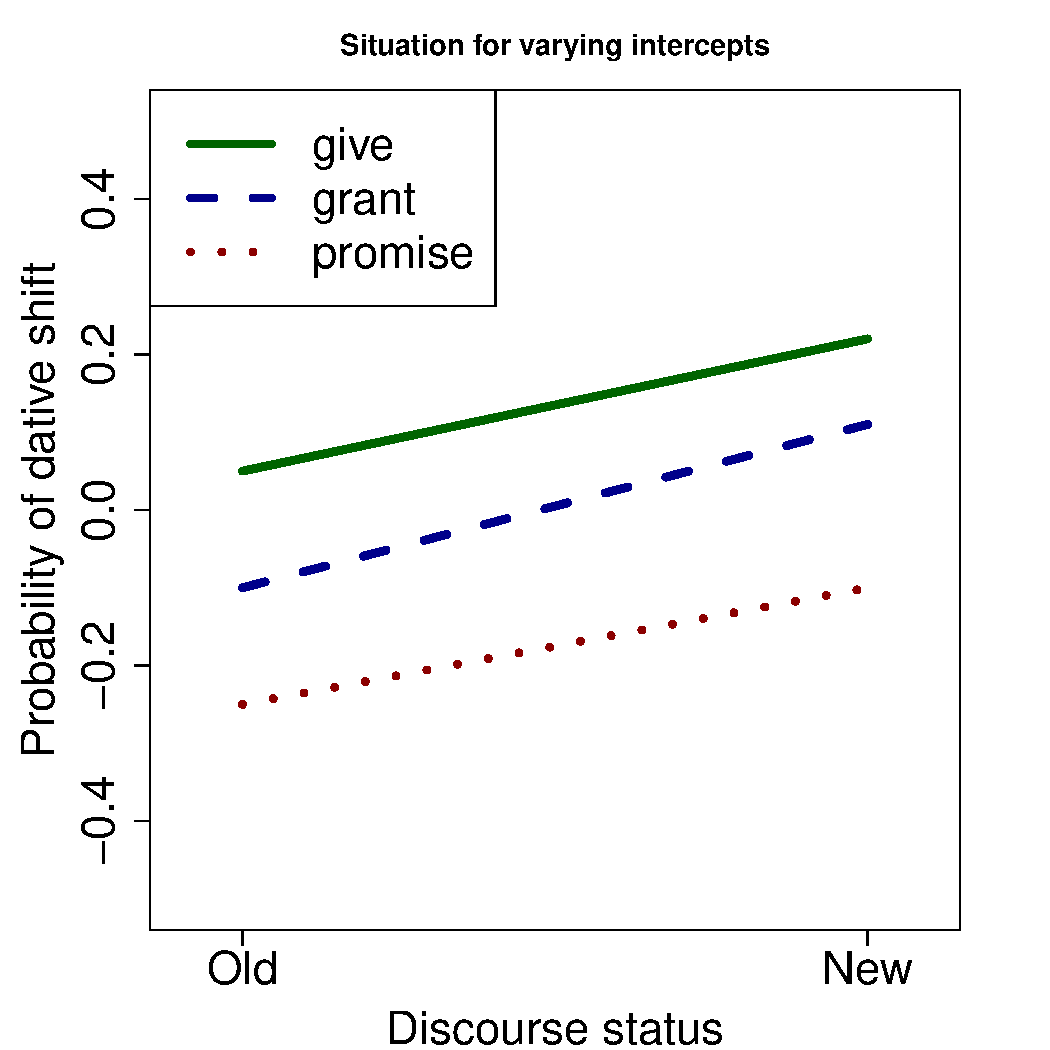
\includegraphics[width=0.5\textwidth]{graphics/var_int}~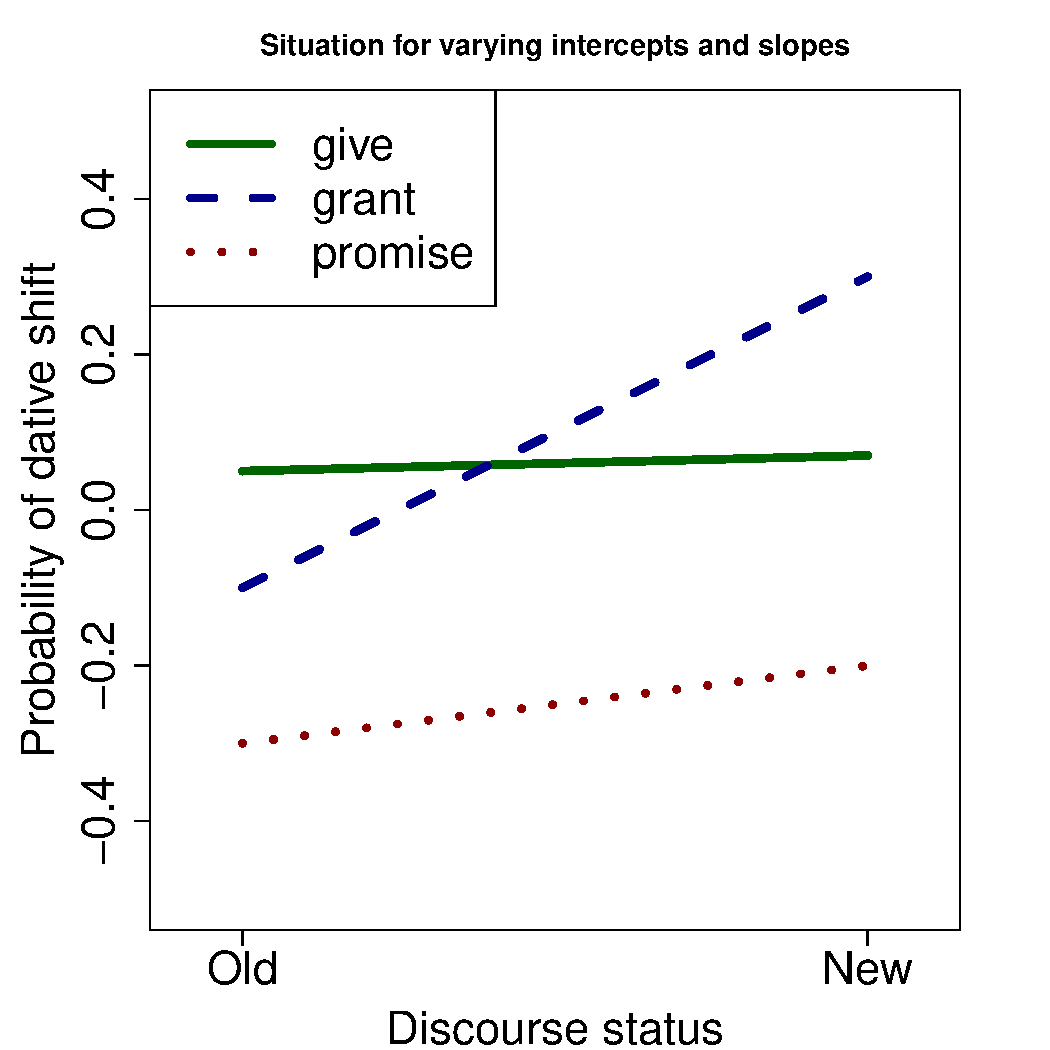
\includegraphics[width=0.5\textwidth]{graphics/var_int_slope}
  \caption{Illustration of fictional data in situations for varying intercepts or varying intercepts and additional varying slopes}
  \label{fig:varintlsope}
\end{figure}

We assume that we are looking at an alternation phenomenon like the dative alternation, wherein we are interested in the probability that, under given circumstances, the dative shift construction is chosen.
In the examination of the data, it turns out that the probability of the dative shift changes for \textit{old} and \textit{new} dative NPs.
The verb lemma also influences the probability of either variant being used.
The situation can now be as in the left or the right panel of Figure~\ref{fig:varintlsope}.
In the situation depicted in the left panel, the overall level in probability changes with the verb lemma, but for each verb lemma, the values change roughly accordingly in exemplars with old and new dative NPs.
Note that the lines are not perfectly parallel because the figure is supposed to be an illustration of a data set rather than a fitted model, and we always expect some chance variation in data sets.
In the situation depicted in the right panel, however, the overall levels are different between lemmas, but the lemma-specific tendencies also vary between exemplars with old and new NPs.
This is actually nothing but an interaction between two factors (verb lemma and givenness), and we could use a fixed-effect interaction to take it into account.
However, if the verb lemma factor is used as a random effect grouping factor, the interaction is modeled as a so-called \textit{random slope}.
In the next section, it is shown how all the different types of data sets discussed so far can be modeled using fixed effects models or, alternatively, using mixed effects models.
Which one is more appropriate will be argued to be better understood as a technical rather than a conceptual question.

